\documentclass[12pt,a4paper]{article}

\usepackage{graphicx}% Include figure files
\usepackage{dcolumn}% Align table columns on decimal point
\usepackage{bm}% bold math
%\usepackage{hyperref}% add hypertext capabilities
%\usepackage[mathlines]{lineno}% Enable numbering of text and display math
%\linenumbers\relax % Commence numbering lines

%\usepackage[showframe,%Uncomment any one of the following lines to test 
%%scale=0.7, marginratio={1:1, 2:3}, ignoreall,% default settings
%%text={7in,10in},centering,
%%margin=1.5in,
%%total={6.5in,8.75in}, top=1.2in, left=0.9in, includefoot,
%%height=10in,a5paper,hmargin={3cm,0.8in},
%]{geometry}

\usepackage{multicol}%Para hacer varias columnas
\usepackage{multicol,caption}
\usepackage{multirow}
\usepackage{cancel}
\usepackage{hyperref}
\hypersetup{
    colorlinks=true,
    linkcolor=blue,
    filecolor=magenta,      
    urlcolor=cyan,
}

\setlength{\topmargin}{-1.0in}
\setlength{\oddsidemargin}{-0.3pc}
\setlength{\evensidemargin}{-0.3pc}
\setlength{\textwidth}{6.75in}
\setlength{\textheight}{9.5in}
\setlength{\parskip}{0.5pc}

\usepackage[utf8]{inputenc}
\usepackage{expl3,xparse,xcoffins,titling,kantlipsum}
\usepackage{graphicx}
\usepackage{xcolor} 
\usepackage{nopageno}
\usepackage{lettrine}
\usepackage{caption}
\renewcommand{\figurename}{Figura}
\usepackage{float}
\renewcommand\refname{Bibliograf\'ia}
\usepackage{amssymb}
\usepackage{amsmath}
\usepackage[rightcaption]{sidecap}
\usepackage[spanish]{babel}

\providecommand{\abs}[1]{\lvert#1\rvert}
\providecommand{\norm}[1]{\lVert#1\rVert}
\newcommand{\dbar}{\mathchar'26\mkern-12mu d}

% CABECERA Y PIE DE PÁGINA %%%%%
\usepackage{fancyhdr}
\pagestyle{fancy}
\fancyhf{}

\begin{document}

\begin{enumerate}
    \item Escribe un programa que aproxime el $\cos{x}$ con una serie de Taylor, donde el programa solicita el argumento y el número de términos de la aproximación, el programa deberá usar una función externa que calcula el factorial, para generar los términos de la serie. Comparar con la función intrínseca $\cos{x}$
    
    \begin{verbatim}
        program taylor
implicit none
real, parameter :: pi = 3.14159265359
integer, parameter :: extra = selected_real_kind(p=24,r=1000)
integer :: i, y, z, n
real(extra), dimension(:), allocatable ::  coss
real(extra) :: x, xx, realcos, scos = 1._extra
!serie de taylor alrededor del 0 (serie de Mclaurin) para aproximar el coseno
!en cualquier valor gracias a la traslación se que usa


write (*,*) "¿Cual es el valor que quieres evaluar?(en radianes)"
read (*,*) x

write (*,*) "¿Cuántos términos quieres?"
read (*,*) n

allocate (coss(0:n))

y = floor(x/pi)
z = modulo(y,2)

if (abs(x) .GT. 2*pi) then !traslación para evitar que algún dato de la serie explote
	xx = x - ((y-z)*pi)

else if (abs(x) .LE.2* pi) then
		xx = x
end if


do i = 1, n, 1 !elementos de la serie
	coss(i) = ((-1)**i) * ((xx**(2*i))/(factorial(2*i)))
end do

do i = 1, n, 1 !suma de todos los elementos
	scos = scos + coss(i)
end do

realcos = cos(x) !coseno "real"
	
write (*,*)"El valor aproximado es : ", scos
write (*,*) "El valor 'real' es : ", realcos

contains
	real function factorial(m)
		implicit none
		integer, intent(IN) :: m
		integer :: i
		real(extra) ::  ans

		ans = 1._extra

		do i = 2, m, 1
			ans = ans * i
		end do

		factorial = ans

	end function factorial
 	
end program taylor
    \end{verbatim}
    
    \begin{figure}[h!]
        \centering
        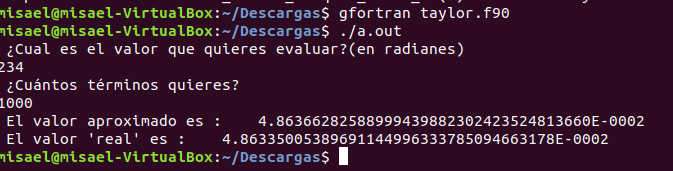
\includegraphics[scale=0.9]{1.1.PNG}
    \end{figure}
    
    \begin{figure}[h!]
        \centering
        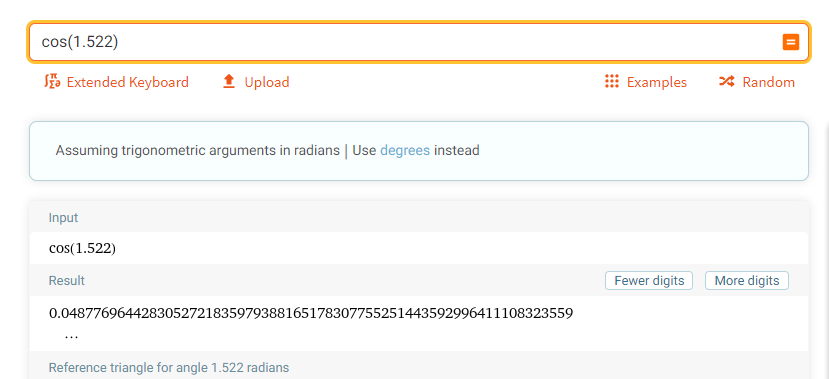
\includegraphics[scale=0.6]{1.2.PNG}
    \end{figure}
    
    \newpage
    
    \item Escribe un programa que genere $10000000$ de números aleatorios entre -1 y 1 en un arreglo y que se los pase a una función junto con un índice (digamos “i”, entero) , la función resolverá para que índice “j” se repite el numero del índice “i” del arreglo, (siempre j > i) con una tolerancia de "0.000001" y con esto determinar cuantos números son generados aleatoriamente para que se vuelva a repetir el elemento i-esimo del arreglo, con esto en el programa principal resuelve la periodicidad del primer numero generado aleatoriamente de los 10 millones , el segundo y el tercero, poner los letreros correspondientes.
    
    el primer programa genera los números aleatorios 
    
    \begin{verbatim}
        program dat
implicit none
integer :: i,j,k
real, dimension(10000000) :: x,z,y

call random_number(x) !genera numeros aleatorios entre 0 y 1

do i=1 , 10000000, 1 !mueve los numeros aleatorios entre -1 y 1
	y(i) = 2*x(i)-1
end do


open(1,file="datos.dat", status="unknown") !carga los datos en un archivo

do i=1, 10000000, 1
	write(1,*)y(i)
end do
close(1)

end program dat

    \end{verbatim}
    
    
    \begin{verbatim}
        program rep
implicit none
integer :: i, j
real, dimension(10000000) :: x

do i=1, 10000000, 1 !bucle para leer datos aleatorios de -1 a 1
  read(*,*) x(i)
end do


do i=1, 10000000, 1!bucles para encontrar los elementos que se repiten
  do j=i, 10000000, 1
    if ((x(i) .lt. x(j)+0.000001) .and. (x(i) .gt. x(j)-0.000001)) then
      write(*,*) "El elemento", x(i),"con índice ",i ,"se repite en el índice", j
    end if
  end do
end do


end program
    \end{verbatim}
    
    este ultimo toma como 1 min en imprimir 1000 datos y suponiendo que el programa imprimirá a una velocidad constante, entonces el programa tardara alrededor de 166 horas
    
    \begin{figure}[h!]
        \centering
        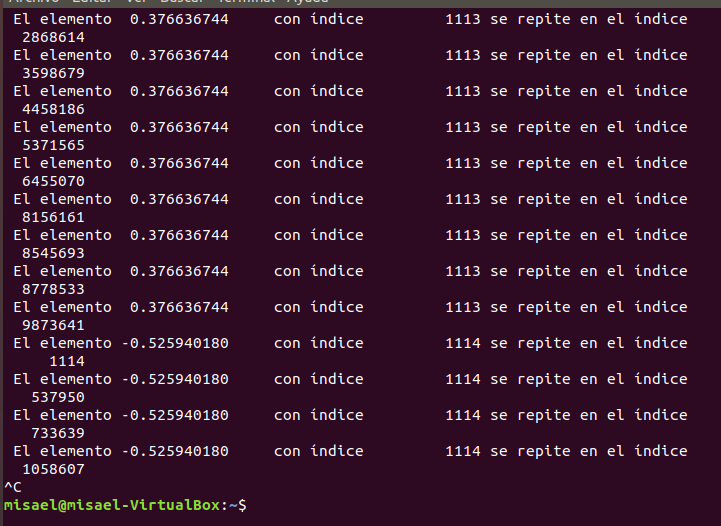
\includegraphics[scale=0.6]{2.1.PNG}
    \end{figure}
    
    \item Utilizando la subrutina RANDOM NUMBER y RANDOM SEED haz un programa que siempre genere los mismos 100 números aleatorios, cuando se corre el programa una y otra vez...
    
    \begin{verbatim}
        program rand2
implicit none
integer :: i,n,seed
real :: x

call initrandomseed()

do i= 1, 100, 1
	call random_number(x)
	write(*,*) x
end do

contains

subroutine initrandomseed()
	integer :: i,n,clock
	integer, dimension(:), allocatable :: seed
	
	call random_seed(size=n)
	allocate(seed(n))
	call system_clock(count=clock)
	seed = 1
	call random_Seed(put=seed)
	deallocate(seed)	
end subroutine initrandomseed

end program rand2

    \end{verbatim}
    
    \begin{figure}[h!]
        \centering
        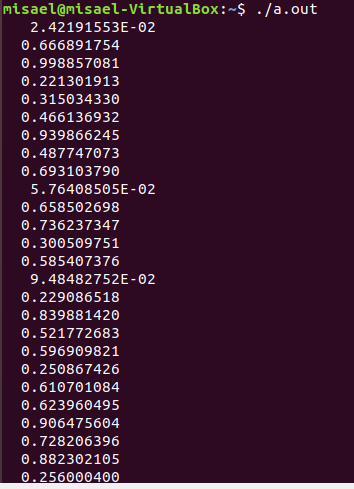
\includegraphics[scale=0.6]{3.1.PNG}
    \end{figure}
    
    \begin{figure}[h!]
        \centering
        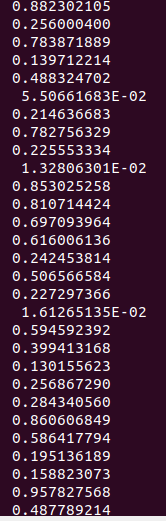
\includegraphics[scale=0.6]{3.2.PNG}
    \end{figure}
    
    \begin{figure}[h!]
        \centering
        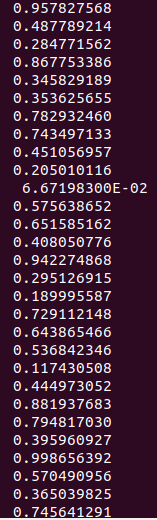
\includegraphics[scale=0.6]{3.3.PNG}
    \end{figure}
    
    \begin{figure}[h!]
        \centering
        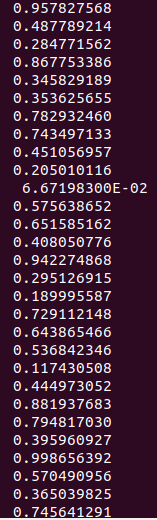
\includegraphics[scale=0.6]{3.3.PNG}
    \end{figure}
    
    \begin{figure}[h!]
        \centering
        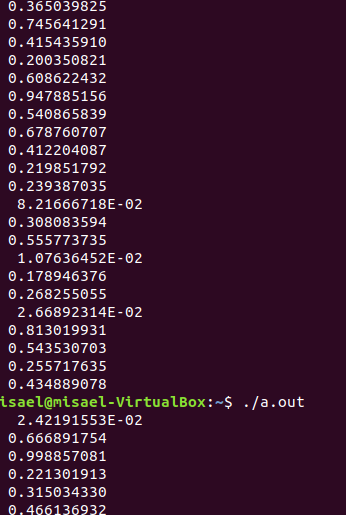
\includegraphics[scale=0.6]{3.4.PNG}
    \end{figure}
    
    \begin{figure}[h!]
        \centering
        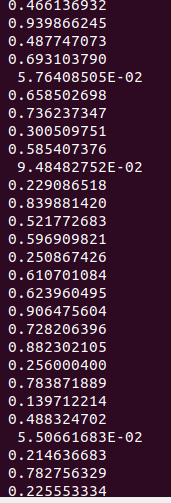
\includegraphics[scale=0.6]{3.5.PNG}
    \end{figure}
    
    \begin{figure}[h!]
        \centering
        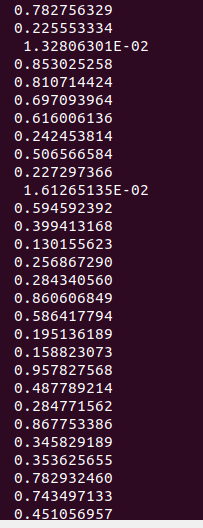
\includegraphics[scale=0.6]{3.6.PNG}
    \end{figure}
    
    \begin{figure}[h!]
        \centering
        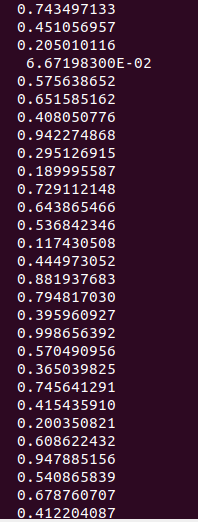
\includegraphics[scale=0.6]{3.7.PNG}
    \end{figure}
    
    \begin{figure}[h!]
        \centering
        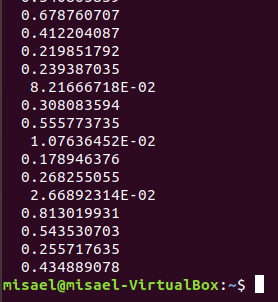
\includegraphics[scale=0.6]{3.8.PNG}
    \end{figure}
\end{enumerate}

\end{document}
